\documentclass[a4paper, 11pt]{article}
\usepackage{comment} % enables the use of multi-line comments (\ifx \fi) 
\usepackage{lipsum} %This package just generates Lorem Ipsum filler text. 
\usepackage{fullpage} % changes the margin
\usepackage{bm}
\usepackage{graphicx}
\usepackage{blindtext}
\usepackage{listings}
\usepackage{amsmath}
\usepackage[colorlinks=true, linkcolor=blue,urlcolor  = blue]{hyperref}
\begin{document}
%Header-Make sure you update this information!!!!
\noindent
Cmpsci585\\
Project Proposal\\
Patrick Carron \\
Raymond Zhu\\
11/11/2016 \\
\begin{center}

\textbf{Predicting Political Party Affiliation from Speech}
\end{center}
\section{Introduction}
We are predicting a speaker's political party affiliation based on the language used in their congressional speeches. Based on our project proposal feedback we decided against scraping presidential campaign speeches and focus on the data which we have already procured. We are using the \href{http://www.cs.cornell.edu/home/llee/data/convote.html}{Congressional speeches dataset} created by Lillian Lee at Cornell. The dataset has been preprocessed somewhat and split into train, dev, and test sets.  We have preformed some exploratory data analysis to ensure high data quality and understand some idiosyncrasies of this data asset. We used Scikit Learn to create a data analysis pipeline so ensure that we have consistency in how the data is being processed while we search for optimal hyper parameters with different classification methods. So far we have implemented a baseline Naive Bayes classifier and a Support Vector Machine classifier with default parameters and found that our results are similar to those described in our literature review.

\section{Dataset}
Number of Documents in Training Set\\
Number of Tokens in Training Set\\
Size of Vocabulary $|V|$ in Training Set\\
Discussion of Dev Set?\\
Discussion of Data Preprocessing (names removed and replaced, spaces inserted, forced to lower case, punctuation remains)\\
Number of Documents in Test Set\\
\section{Software and Code Structure}
We were able to read in our data files and simultaneously parse the file name to record the political party of the speaker. Since the dataset was already split into train, test, and development sets, we read in each folder separately and made certain that no test data intermingled with either the training or development sets.  After reviewing the data set and reading documentation on several natural language processing libraries, we decided to use Scikit learn.  Specifically, Scikit learn offers the ability to create data pipelines and transform our feature vectors easily and consistently while preforming a set of experiments. Within our pipeline, we are using Scikit Learn's feature extraction library to create word count vectors and train our classifiers. This package will allow us to test the impact of TF-IDF weighting on our classification accuracy, along with searching over different length language models to determine which is most predictive. We had to alter our code so that we could recover basic word count and vocabulary statistics, and we printed out both the most commonly used terms and the least frequently used terms to ensure that we are using the data structures correctly.  Finally, we used matplotlib to create a visualization of Zipf's law on our training corpus.

\section{Baseline Algorithm}
Naive Bayes, assumptions and Results\\
-Multinomial NB because independent party\\
-Multinomial NB also allows for smoothing in sclearn\\
SVD results as well\\
Discuss accuracies.\\
\section{Timeline}
Implement Cross validation code for each classifier 11/19\\
Write code to create cv graphs over range of hyper parameters 11/26\\
Draft of Poster and all exhibits 12/3\\
Draft of Final paper 12/7\\
Finalize Poster 12/10\\
Final Draft of Paper 12/10\\
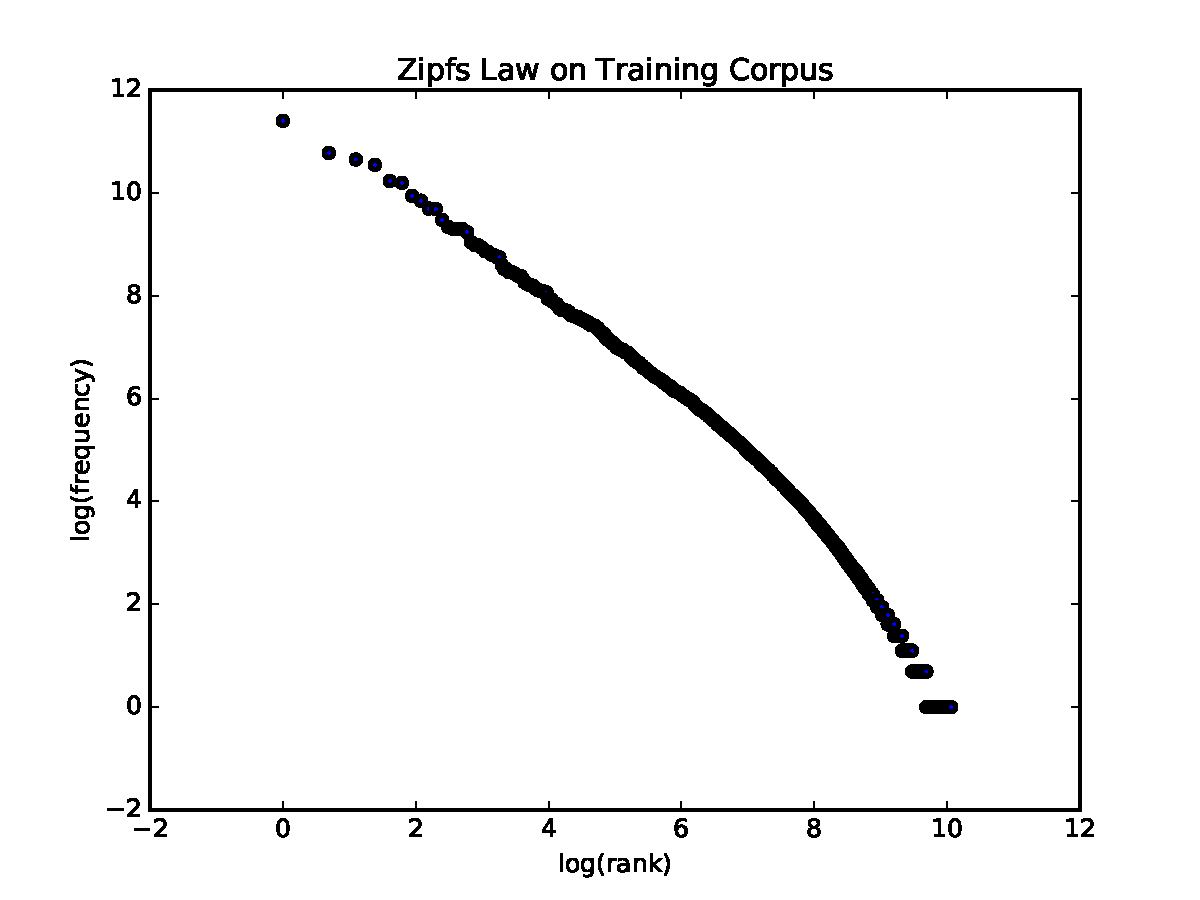
\includegraphics[scale=.5]{zipfslaw.pdf}
\end{document}